\chapter{Schémas de Lewis et géométrie des molécules}\label{ch:g10:lewis-and-shape}

Une \omterm{def:g7:atoms-and-molecules:molecule}{molécule} de dioxyde de carbone est linéaire~; une \omterm{def:g7:atoms-and-molecules:molecule}{molécule} d'eau est
coudée. Cette seule différence de forme est l'une des raisons pour
lesquelles l'eau, dont les \omterm{def:g7:atoms-and-molecules:molecule}{molécules} sont plus légères que celles du
dioxyde de carbone, est liquide à température ambiante alors que le
dioxyde de carbone est un gaz. Dans une \omterm{def:g7:atoms-and-molecules:molecule}{molécule}, les \omterm{def:g7:atoms-and-molecules:atom}{atomes} sont unis
par des \omterm{def:g9:inside-the-atom:nucleus}{électrons} mis en commun, et la façon dont ces \omterm{def:g9:inside-the-atom:nucleus}{électrons} sont
partagés décide de la forme. Ce chapitre dessine les \omterm{def:g9:inside-the-atom:nucleus}{électrons} mis en
commun et en déduit la géométrie.

\begin{recall}
Les \omterm{def:g10:electron-shells:valence}{électrons de valence} sont ceux de la \omterm{def:g10:electron-shells:configuration}{couche} externe~; les \omterm{def:g7:atoms-and-molecules:atom}{atomes}
tendent à acquérir la configuration d'un \omterm{def:g10:electron-shells:family}{gaz noble}, huit \omterm{def:g9:inside-the-atom:nucleus}{électrons} sur
la \omterm{def:g10:electron-shells:configuration}{couche} externe (\omterm{def:g10:electron-shells:octet}{règle de l'octet}) ou deux pour l'hydrogène (\omterm{def:g10:electron-shells:octet}{règle du
duet}) (\cref{ch:g10:electron-shells}). Les modèles moléculaires
représentent les \omterm{def:g7:atoms-and-molecules:atom}{atomes} par des boules et les liaisons par des bâtonnets
(\cref{ch:g7:atoms-and-molecules}).
\end{recall}

\section{La liaison covalente}

\begin{definition}[Liaison covalente]\label{def:g10:lewis-and-shape:covalent-bond}
Une \emph{liaison covalente}\index{liaison covalente} est une paire
d'\omterm{def:g9:inside-the-atom:nucleus}{électrons} mise en commun par deux \omterm{def:g7:atoms-and-molecules:atom}{atomes}~; chaque \omterm{def:g7:atoms-and-molecules:atom}{atome} fournit en
général un \omterm{def:g9:inside-the-atom:nucleus}{électron} de la paire. Les deux \omterm{def:g7:atoms-and-molecules:atom}{atomes} comptent cette paire
commune dans leur \omterm{def:g10:electron-shells:configuration}{couche} externe, ce qui permet à chacun d'atteindre un
duet ou un octet.
\end{definition}

\begin{definition}[Doublets liants et doublets non liants]\label{def:g10:lewis-and-shape:lone-pair}
Dans une \omterm{def:g7:atoms-and-molecules:molecule}{molécule}, les \omterm{def:g10:electron-shells:valence}{électrons de valence} de chaque \omterm{def:g7:atoms-and-molecules:atom}{atome} sont
regroupés par paires, appelées doublets. Un
\emph{doublet liant}\index{doublet liant} est mis en commun par deux
\omterm{def:g7:atoms-and-molecules:atom}{atomes} et forme une \omterm{def:g10:lewis-and-shape:covalent-bond}{liaison covalente}~; un
\emph{doublet non liant}\index{doublet non liant} appartient à un seul
\omterm{def:g7:atoms-and-molecules:atom}{atome} et ne participe à aucune liaison.
\end{definition}

\begin{proposition}[Combien de liaisons un atome forme]\label{prop:g10:lewis-and-shape:valence}
Un \omterm{def:g7:atoms-and-molecules:atom}{atome} forme autant de \omterm{def:g10:lewis-and-shape:covalent-bond}{liaisons covalentes} qu'il lui manque d'\omterm{def:g9:inside-the-atom:nucleus}{électrons}
pour compléter son duet ou son octet~:
\begin{center}
\small
\begin{tabular}{lcccc}
\hline
\omterm{def:g7:atoms-and-molecules:atom}{atome} & \omterm{def:g10:electron-shells:valence}{électrons de valence} & liaisons & \omterm{def:g10:lewis-and-shape:lone-pair}{doublets non liants} & exemple \\
\hline
H & 1 & 1 & 0 & \ce{H2} \\
C & 4 & 4 & 0 & \ce{CH4} \\
N & 5 & 3 & 1 & \ce{NH3} \\
O & 6 & 2 & 2 & \ce{H2O} \\
Cl & 7 & 1 & 3 & \ce{HCl} \\
\hline
\end{tabular}
\end{center}
\end{proposition}

\section{Les schémas de Lewis}

\begin{definition}[Schéma de Lewis]\label{def:g10:lewis-and-shape:lewis-structure}
Le \emph{schéma de Lewis}\index{schema de lewis@schéma de Lewis} d'une \omterm{def:g7:atoms-and-molecules:molecule}{molécule}
représente ses \omterm{def:g7:atoms-and-molecules:atom}{atomes} par leurs symboles, chaque \omterm{def:g10:lewis-and-shape:lone-pair}{doublet liant} par un
trait entre deux \omterm{def:g7:atoms-and-molecules:atom}{atomes} et chaque \omterm{def:g10:lewis-and-shape:lone-pair}{doublet non liant} par un trait (ou une
paire de points) placé à côté de son \omterm{def:g7:atoms-and-molecules:atom}{atome}.
\end{definition}

\begin{definition}[Liaisons doubles et triples]\label{def:g10:lewis-and-shape:multiple-bond}
Deux \omterm{def:g7:atoms-and-molecules:atom}{atomes} peuvent mettre en commun deux doublets, une \emph{liaison
double}\index{liaison double}, représentée par deux traits, ou trois
doublets, une \emph{liaison triple}\index{liaison triple}, représentée
par trois traits.
\end{definition}

\begin{method}[Établir un schéma de Lewis]\label{met:g10:lewis-and-shape:draw}
\begin{enumerate}
  \item Additionner les \omterm{def:g10:electron-shells:valence}{électrons de valence} de tous les \omterm{def:g7:atoms-and-molecules:atom}{atomes}, et
        diviser par deux pour obtenir le nombre de doublets.
  \item Relier les \omterm{def:g7:atoms-and-molecules:atom}{atomes} par des liaisons simples (l'hydrogène, qui ne
        forme qu'une liaison, est toujours à l'extérieur~; le carbone est
        en général central).
  \item Placer les doublets restants comme \omterm{def:g10:lewis-and-shape:lone-pair}{doublets non liants}, d'abord
        sur les \omterm{def:g7:atoms-and-molecules:atom}{atomes} extérieurs, pour compléter leurs octets.
  \item Si un \omterm{def:g7:atoms-and-molecules:atom}{atome} n'a toujours pas d'octet, transformer un \omterm{def:g10:lewis-and-shape:lone-pair}{doublet non
        liant} d'un voisin en un deuxième (ou un troisième) \omterm{def:g10:lewis-and-shape:lone-pair}{doublet liant}.
  \item Vérifier~: chaque hydrogène a 2 \omterm{def:g9:inside-the-atom:nucleus}{électrons}, chaque autre \omterm{def:g7:atoms-and-molecules:atom}{atome} 8,
        et tous les doublets ont été utilisés.
\end{enumerate}
\end{method}

\begin{example}[Le dioxyde de carbone]\label{ex:g10:lewis-and-shape:co2}
\ce{CO2}~: $4 + 2 \times 6 = 16$ \omterm{def:g10:electron-shells:valence}{électrons de valence}, 8 doublets. Les
liaisons simples \ce{O-C-O} utilisent 2 doublets~; 6 \omterm{def:g10:lewis-and-shape:lone-pair}{doublets non liants}
complètent les oxygènes, mais le carbone n'a alors que 4 \omterm{def:g9:inside-the-atom:nucleus}{électrons}. En
transformant un \omterm{def:g10:lewis-and-shape:lone-pair}{doublet non liant} de chaque oxygène en \omterm{def:g10:lewis-and-shape:lone-pair}{doublet liant}, on
obtient deux \omterm{def:g10:lewis-and-shape:multiple-bond}{liaisons doubles}~: chaque \omterm{def:g7:atoms-and-molecules:atom}{atome} a maintenant un octet.
\end{example}

\begin{omfigure}
\setchemfig{atom sep=2.0em}
\begin{tabular}{cccccc}
\chemfig{H-H} & \chemfig{H-\charge{0=\:,90=\:,270=\:}{Cl}} & \chemfig{H-\charge{90=\:,270=\:}{O}-H} &
\chemfig{H-\charge{90=\:}{N}(-[6]H)-H} & \chemfig{H-C(-[2]H)(-[6]H)-H} &
\chemfig{\charge{135=\:,225=\:}{O}=C=\charge{45=\:,315=\:}{O}} \\[4pt]
\small \ce{H2} & \small \ce{HCl} & \small \ce{H2O} & \small \ce{NH3} & \small \ce{CH4} & \small \ce{CO2} \\[10pt]
\chemfig{\charge{180=\:}{N}~\charge{0=\:}{N}} & \chemfig{\charge{135=\:,225=\:}{O}=\charge{45=\:,315=\:}{O}} &
\chemfig{C(-[3]H)(-[5]H)=C(-[1]H)-[7]H} & \chemfig{H-C~\charge{0=\:}{N}} &
\chemfig{H-C(-[6]H)=\charge{45=\:,315=\:}{O}} & \\[4pt]
\small \ce{N2} & \small \ce{O2} & \small \ce{C2H4} & \small \ce{HCN} & \small méthanal \ce{CH2O} &
\end{tabular}

{\small \omterm{def:g10:lewis-and-shape:lewis-structure}{Schémas de Lewis} de onze \omterm{def:g7:atoms-and-molecules:molecule}{molécules}. Chaque \omterm{def:g7:atoms-and-molecules:atom}{atome} autre que
l'hydrogène est entouré de quatre doublets (liants et non liants)~: un
octet.}
\end{omfigure}

\section{La géométrie des molécules}

\begin{proposition}[Les doublets s'éloignent le plus possible les uns des autres]\label{prop:g10:lewis-and-shape:shape}
Autour d'un \omterm{def:g7:atoms-and-molecules:atom}{atome} central, les groupes d'\omterm{def:g9:inside-the-atom:nucleus}{électrons} --- chaque liaison
simple, double ou triple, et chaque \omterm{def:g10:lewis-and-shape:lone-pair}{doublet non liant} --- se repoussent
et se placent aussi loin que possible les uns des autres. La géométrie
de la \omterm{def:g7:atoms-and-molecules:molecule}{molécule} en découle~:
\begin{center}
\small
\begin{tabular}{llll}
\hline
groupes autour du centre & dont \omterm{def:g10:lewis-and-shape:lone-pair}{doublets non liants} & géométrie & exemple \\
\hline
2 & 0 & linéaire, angle \ang{180} & \ce{CO2}, \ce{HCN} \\
3 & 0 & triangulaire plane, angle \ang{120} & \ce{CH2O}, \ce{C2H4} \\
4 & 0 & tétraédrique, angle \ang{109.5} & \ce{CH4} \\
4 & 1 & pyramidale & \ce{NH3} \\
4 & 2 & coudée & \ce{H2O} \\
\hline
\end{tabular}
\end{center}
\end{proposition}
\admitted

\begin{remark}[D'où vient cette règle]\label{rem:g10:lewis-and-shape:vsepr}
Cette règle est un modèle, et elle fonctionne remarquablement bien pour
les petites \omterm{def:g7:atoms-and-molecules:molecule}{molécules}~; elle est précisée, et en partie expliquée, dans
le volume de première année d'université. Les \omterm{def:g10:lewis-and-shape:lone-pair}{doublets non liants}
prennent un peu plus de place que les \omterm{def:g10:lewis-and-shape:lone-pair}{doublets liants}~: l'angle de
l'ammoniac (\ang{106.7}) et celui de l'eau (\ang{104.5}) sont un peu
plus petits que les \ang{109.5} du méthane.
\end{remark}

\begin{omfigure}
\begin{tikzpicture}[font=\small]
  % methane, tetrahedral, in perspective
  \begin{scope}
    \node[aC] (c) at (0,0) {};
    \node[aH, minimum size=3.6mm] (hb) at (0.3,-0.12) {};
    \node[aH] (h1) at (0,1.05) {};
    \node[aH] (h2) at (-1.0,-0.45) {};
    \node[aH] (h3) at (0.72,-0.5) {};
    \begin{scope}[on background layer]
      \foreach \h in {h1,h2,h3,hb} \draw[bond] (c.center) -- (\h.center);
    \end{scope}
    \node[aC] at (0,0) {};
    \node at (0,-1.35) {méthane~: tétraèdre};
    \node[font=\footnotesize] at (-0.55,0.55) {\ang{109.5}};
  \end{scope}
  % ammonia, pyramid
  \begin{scope}[xshift=4.2cm]
    \fill[omDef!25] (0,0.2) ellipse (0.18 and 0.45);
    \node[font=\scriptsize, omDef] at (0,1.0) {doublet non liant};
    \node[aN] (n) at (0,0) {};
    \node[aH] (h1) at (-0.95,-0.5) {};
    \node[aH] (h2) at (0.7,-0.55) {};
    \node[aH, minimum size=3.6mm] (h3) at (0.25,-0.2) {};
    \begin{scope}[on background layer]
      \foreach \h in {h1,h2,h3} \draw[bond] (n.center) -- (\h.center);
    \end{scope}
    \node[aN] at (0,0) {};
    \node at (0,-1.35) {ammoniac~: pyramide};
  \end{scope}
  % water, bent
  \begin{scope}[xshift=8.4cm]
    \fill[omDef!25, rotate=25] (0,0.2) ellipse (0.16 and 0.42);
    \fill[omDef!25, rotate=-25] (0,0.2) ellipse (0.16 and 0.42);
    \node[aO] (o) at (0,0) {};
    \node[aH] (h1) at (-0.8,-0.58) {};
    \node[aH] (h2) at (0.8,-0.58) {};
    \begin{scope}[on background layer]
      \draw[bond] (o.center) -- (h1.center); \draw[bond] (o.center) -- (h2.center);
    \end{scope}
    \node[aO] at (0,0) {};
    \draw[black!60] (-0.32,-0.23) arc[start angle=216, end angle=324, radius=0.4];
    \node[font=\footnotesize] at (0,-0.65) {\ang{104.5}};
    \node at (0,-1.35) {eau~: coudée};
  \end{scope}
  % carbon dioxide, linear
  \begin{scope}[xshift=12.0cm]
    \node[aO] (a) at (-0.8,0) {}; \node[aC] (c) at (0,0) {}; \node[aO] (b) at (0.8,0) {};
    \begin{scope}[on background layer]
      \foreach \d in {-1.6,1.6} {
        \draw[bond, line width=1.1pt] ([yshift=\d pt]a.center) -- ([yshift=\d pt]c.center);
        \draw[bond, line width=1.1pt] ([yshift=\d pt]c.center) -- ([yshift=\d pt]b.center);}
    \end{scope}
    \node at (0,-1.35) {dioxyde de carbone~: linéaire};
  \end{scope}
\end{tikzpicture}

{\small Géométrie de quatre \omterm{def:g7:atoms-and-molecules:molecule}{molécules} (\omterm{def:g10:lewis-and-shape:lone-pair}{doublets non liants} figurés par
des lobes grisés).
% ledger: ang:H2O, ang:NH3
Le méthane est un tétraèdre, l'ammoniac une pyramide, l'eau est coudée,
le dioxyde de carbone linéaire.}
\end{omfigure}

\begin{omfigure}
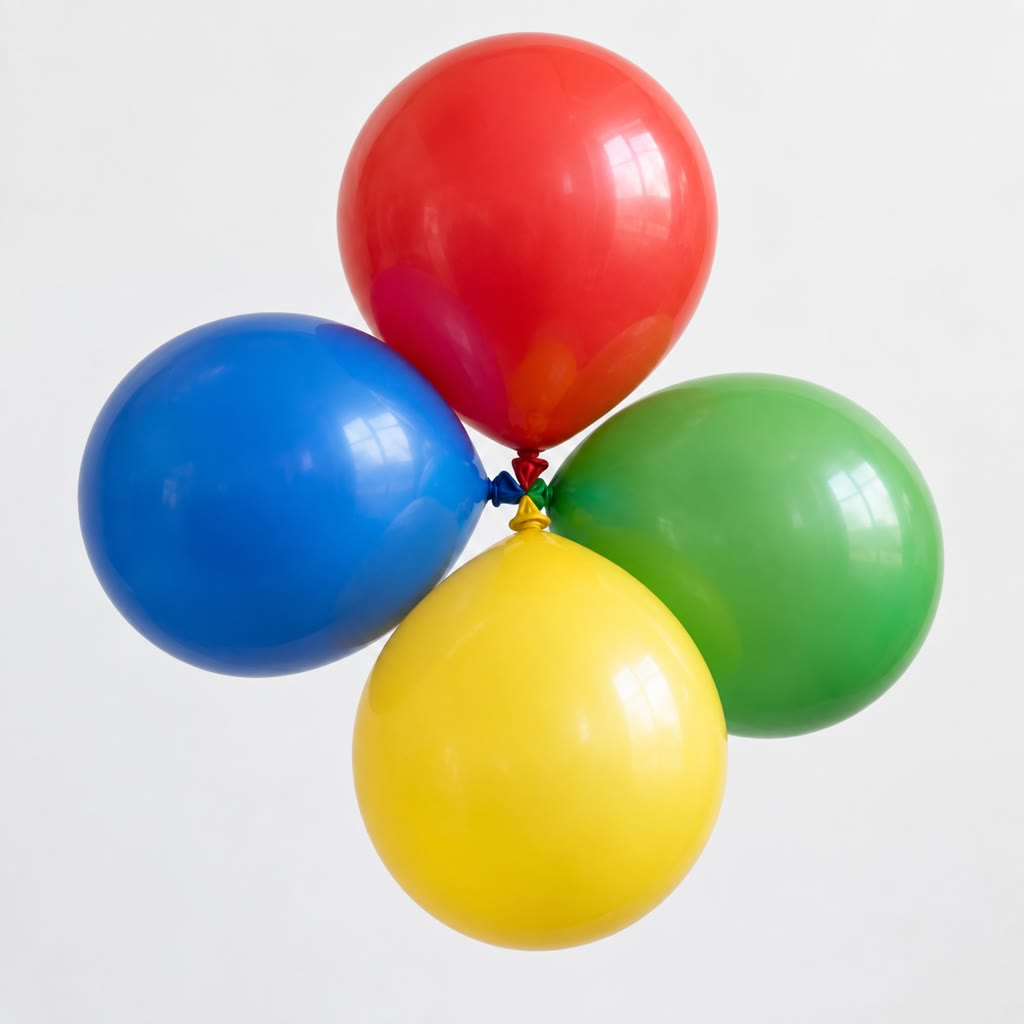
\includegraphics[width=0.38\linewidth]{images/book1/ai/g10-balloons-tetrahedron.jpg}

{\small Quatre ballons attachés ensemble se repoussent le plus loin
possible les uns des autres~; dans l'espace, ils pointent vers les
sommets d'un tétraèdre, comme les quatre doublets autour d'un \omterm{def:g7:atoms-and-molecules:atom}{atome} de
carbone.}
\end{omfigure}

\section{Représenter les molécules dans l'espace}

\begin{notation}[Triangles pleins et triangles hachurés]\label{not:g10:lewis-and-shape:wedge}
Pour dessiner une \omterm{def:g7:atoms-and-molecules:molecule}{molécule} dans l'espace sur une feuille plane, une
liaison située dans le plan de la feuille est un trait simple, une
liaison qui pointe vers le lecteur un triangle plein, et une liaison qui
s'éloigne un triangle hachuré. On dessine alors le méthane comme
ci-dessous~: deux liaisons dans le plan, l'une vers le lecteur et l'autre
vers l'arrière.
\begin{center}
\chemfig{C(-[2]H)(-[4]H)(<[7]H)(<:[5]H)}
\end{center}
\end{notation}

\section{Exercices}

\begin{exercise}[$\star$]\label{exo:g10:lewis-and-shape:1}
Qu'est-ce qu'une \omterm{def:g10:lewis-and-shape:covalent-bond}{liaison covalente}~? Qu'est-ce qu'un \omterm{def:g10:lewis-and-shape:lone-pair}{doublet non liant}~?
\end{exercise}

\begin{exercise}[$\star$]\label{exo:g10:lewis-and-shape:2}
Combien de \omterm{def:g10:lewis-and-shape:covalent-bond}{liaisons covalentes} l'hydrogène, le carbone, l'azote et
l'oxygène forment-ils en général~? Expliquer à l'aide des \omterm{def:g10:electron-shells:octet}{règles de
l'octet} et du duet.
\end{exercise}

\begin{exercise}[$\star$]\label{exo:g10:lewis-and-shape:3}
Établir le \omterm{def:g10:lewis-and-shape:lewis-structure}{schéma de Lewis} du chlorure d'hydrogène, \ce{HCl}, et compter
les \omterm{def:g9:inside-the-atom:nucleus}{électrons} autour du chlore.
\end{exercise}

\begin{exercise}[$\star$]\label{exo:g10:lewis-and-shape:4}
Combien d'\omterm{def:g10:electron-shells:valence}{électrons de valence}, au total, la \omterm{def:g7:atoms-and-molecules:molecule}{molécule} \ce{NH3}
possède-t-elle~? Combien de doublets~?
\end{exercise}

\begin{exercise}[$\star$]\label{exo:g10:lewis-and-shape:5}
Donner la géométrie de \ce{CH4}, \ce{NH3}, \ce{H2O} et \ce{CO2}.
\end{exercise}

\begin{exercise}[$\star\star$]\label{exo:g10:lewis-and-shape:6}
Établir le \omterm{def:g10:lewis-and-shape:lewis-structure}{schéma de Lewis} du sulfure d'hydrogène, \ce{H2S} (le soufre
est dans le groupe de l'oxygène), et prévoir sa géométrie.
\end{exercise}

\begin{exercise}[$\star\star$]\label{exo:g10:lewis-and-shape:7}
Établir le \omterm{def:g10:lewis-and-shape:lewis-structure}{schéma de Lewis} du diazote, \ce{N2}, en suivant la méthode pas
à pas.
\end{exercise}

\begin{exercise}[$\star\star$]\label{exo:g10:lewis-and-shape:8}
Établir le \omterm{def:g10:lewis-and-shape:lewis-structure}{schéma de Lewis} du méthanol, \ce{CH3OH}, et donner la
géométrie autour du carbone et autour de l'oxygène.
\end{exercise}

\begin{exercise}[$\star\star$]\label{exo:g10:lewis-and-shape:9}
Expliquer pourquoi \ce{CO2} est linéaire et \ce{H2O} coudée, alors que
toutes deux ont un \omterm{def:g7:atoms-and-molecules:atom}{atome} central lié à deux autres.
\end{exercise}

\begin{exercise}[$\star\star$]\label{exo:g10:lewis-and-shape:10}
Établir le \omterm{def:g10:lewis-and-shape:lewis-structure}{schéma de Lewis} de l'éthène, \ce{C2H4}, et donner la
géométrie autour de chaque \omterm{def:g7:atoms-and-molecules:atom}{atome} de carbone.
\end{exercise}

\begin{exercise}[$\star\star$]\label{exo:g10:lewis-and-shape:11}
Établir le \omterm{def:g10:lewis-and-shape:lewis-structure}{schéma de Lewis} du tétrachlorométhane, \ce{CCl4}, et prévoir
sa géométrie.
\end{exercise}

\begin{exercise}[$\star\star\star$]\label{exo:g10:lewis-and-shape:12}
Deux \omterm{def:g7:atoms-and-molecules:molecule}{molécules} ont pour formule \ce{C2H6O}. Établir un \omterm{def:g10:lewis-and-shape:lewis-structure}{schéma de Lewis}
pour chacune (l'une possède une liaison O--H, l'autre un enchaînement
C--O--C).
\end{exercise}

\begin{exercise}[$\star\star\star$]\label{exo:g10:lewis-and-shape:13}
Expliquer, à l'aide des \omterm{def:g10:lewis-and-shape:lone-pair}{doublets non liants}, pourquoi l'angle de
l'ammoniac (\ang{106.7}) est plus petit que celui du méthane
(\ang{109.5}), et celui de l'eau (\ang{104.5}) plus petit encore.
\end{exercise}

\begin{exercise}[$\star\star\star$]\label{exo:g10:lewis-and-shape:14}
Établir le \omterm{def:g10:lewis-and-shape:lewis-structure}{schéma de Lewis} du cyanure d'hydrogène, \ce{HCN}, et celui du
méthanal, \ce{CH2O}, et donner leurs géométries.
\end{exercise}

\begin{exercise}[$\star\star\star$]\label{exo:g10:lewis-and-shape:15}
L'ozone, \ce{O3}, est une chaîne de trois \omterm{def:g7:atoms-and-molecules:atom}{atomes} d'oxygène. Compter ses
doublets de valence et établir un \omterm{def:g10:lewis-and-shape:lewis-structure}{schéma de Lewis} dans lequel chaque
oxygène a un octet (une \omterm{def:g10:lewis-and-shape:multiple-bond}{liaison double}, une liaison simple). Prévoir si
la \omterm{def:g7:atoms-and-molecules:molecule}{molécule} est linéaire ou coudée.
\end{exercise}

\section{Problème~: une molécule dans un cube}

\begin{problem}[{Problème du week-end --- concevoir les boules de carbone
d'une boîte de modèles moléculaires~: à quel angle percer les trous~?}]
\label{pb:g10:lewis-and-shape:1}
% ledger: ang:H2O, ang:NH3
Une entreprise fabrique des boîtes de modèles moléculaires. Les boules
noires de carbone doivent avoir quatre trous, pour que le méthane,
l'éthane et les autres \omterm{def:g7:atoms-and-molecules:molecule}{molécules} carbonées aient la bonne forme.
L'ingénieure utilise une astuce~: un tétraèdre régulier s'inscrit dans
un cube, ses quatre sommets sur quatre sommets du cube, jamais deux sur
une même arête.

\medskip
\noindent\textbf{Partie I --- Les \omterm{def:g10:lewis-and-shape:lewis-structure}{schémas de Lewis}.}
\begin{enumerate}
  \item Établir les \omterm{def:g10:lewis-and-shape:lewis-structure}{schémas de Lewis} du méthane \ce{CH4}, de l'ammoniac
        \ce{NH3} et de l'eau \ce{H2O}.
  \item Combien de groupes d'\omterm{def:g9:inside-the-atom:nucleus}{électrons} entourent l'\omterm{def:g7:atoms-and-molecules:atom}{atome} central dans
        chacune~?
  \item Combien d'entre eux sont des \omterm{def:g10:lewis-and-shape:lone-pair}{doublets non liants}~?
  \item Pourquoi une boule de carbone a-t-elle besoin de quatre trous, et
        une boule d'oxygène (pour l'eau) de deux seulement~?
  \item Un modèle d'éthane, \ce{C2H6}, utilise deux boules de carbone.
        Établir son \omterm{def:g10:lewis-and-shape:lewis-structure}{schéma de Lewis}. Combien de bâtonnets relient les deux
        boules de carbone, et combien de boules d'hydrogène faut-il~?
\end{enumerate}

\medskip
\noindent\textbf{Partie II --- Les géométries.}
\begin{enumerate}[resume]
  \item Donner la géométrie de chacune des trois \omterm{def:g7:atoms-and-molecules:molecule}{molécules}.
  \item Les angles mesurés valent \ang{106.7} dans l'ammoniac et
        \ang{104.5} dans l'eau. Expliquer pourquoi ils sont plus petits
        que l'angle du méthane.
  \item Pourquoi la boule d'oxygène de l'eau ne peut-elle pas être
        simplement une boule de carbone dont deux trous restent vides, si
        la boîte doit montrer le vrai angle~?
  \item Dans le dioxyde de carbone, l'\omterm{def:g7:atoms-and-molecules:atom}{atome} de carbone forme deux
        \omterm{def:g10:lewis-and-shape:multiple-bond}{liaisons doubles}. Quel angle doit les séparer dans un modèle~?
\end{enumerate}

\medskip
\noindent\textbf{Partie III --- Le cube.}
Soit un cube d'arête $a$. L'\omterm{def:g7:atoms-and-molecules:atom}{atome} de carbone est en son centre~; les
quatre \omterm{def:g7:atoms-and-molecules:atom}{atomes} d'hydrogène occupent quatre sommets du cube, jamais deux
sur une même arête.
\begin{enumerate}[resume]
  \item Montrer que deux quelconques de ces \omterm{def:g7:atoms-and-molecules:atom}{atomes} d'hydrogène sont aux
        deux extrémités d'une diagonale d'une face du cube. À l'aide du
        théorème de Pythagore, calculer la distance qui les sépare en
        fonction de $a$.
  \item La grande diagonale du cube (d'un sommet au sommet opposé) a
        pour longueur $a\sqrt{3}$. En déduire la distance entre l'\omterm{def:g7:atoms-and-molecules:atom}{atome} de
        carbone et un \omterm{def:g7:atoms-and-molecules:atom}{atome} d'hydrogène.
  \item On prend $a = \qty{1}{cm}$ dans un modèle~: donner les deux
        distances en centimètres, au centième près.
  \item Pourquoi les quatre distances C--H sont-elles égales~?
\end{enumerate}

\medskip
\noindent\textbf{Partie IV --- L'angle.}
L'\omterm{def:g7:atoms-and-molecules:atom}{atome} de carbone C et deux \omterm{def:g7:atoms-and-molecules:atom}{atomes} d'hydrogène H$_1$, H$_2$ forment un
triangle isocèle. Soit M le milieu de H$_1$H$_2$.
\begin{enumerate}[resume]
  \item Expliquer pourquoi le triangle C\,M\,H$_1$ est rectangle en M.
  \item Calculer, dans ce triangle rectangle, le sinus de l'angle
        $\widehat{\text{M\,C\,H}_1}$, moitié de l'angle H--C--H.
  \item En déduire le demi-angle, puis l'angle H--C--H, au dixième de
        degré près.
  \item Comparer avec l'angle donné dans le tableau de ce chapitre.
  \item Donner l'angle selon lequel les trous d'une boule de carbone
        doivent être percés.
\end{enumerate}
\end{problem}
